%%%%%%%%%%%%%%%%%%%%%%%%%%%%%%%%%%%%%%%%%
% Short Sectioned Assignment
% LaTeX Template
% Version 1.0 (5/5/12)
%
% This template has been downloaded from:
% http://www.LaTeXTemplates.com
%
% Original author:
% Frits Wenneker (http://www.howtotex.com)
% License:
% CC BY-NC-SA 3.0 (http://creativecommons.org/licenses/by-nc-sa/3.0/)
%
%%%%%%%%%%%%%%%%%%%%%%%%%%%%%%%%%%%%%%%%%

%----------------------------------------------------------------------------------------
%	PACKAGES AND OTHER DOCUMENT CONFIGURATIONS
%----------------------------------------------------------------------------------------

\documentclass[paper=a4, fontsize=10pt, font=arial]{scrartcl} % A4 paper and 11pt font size
\usepackage[T1]{fontenc} % Use 8-bit encoding that has 256 glyphs
\usepackage{fourier} % Use the Adobe Utopia font for the document - comment this line to return to the LaTeX default
\usepackage[english]{babel} % English language/hyphenation
\usepackage{amsmath,amsfonts,amsthm} % Math packages
\usepackage{url}
\usepackage{sectsty} % Allows customizing section commands
\allsectionsfont{\centering \normalfont\scshape} % Make all sections centered, the default font and small caps
%\graphicspath{ {figures/} }
\usepackage{geometry}
\usepackage{float}
\usepackage{graphicx}
\usepackage{caption}
\usepackage{subcaption}
\usepackage{cite}
\usepackage{fancyhdr} % Custom headers and footers
%\usepackage{movie15}
%\bibliographystyle{unsrt}
\pagestyle{fancyplain} % Makes all pages in the document conform to the custom headers and footers
\fancyhead{} % No page header - if you want one, create it in the same way as the footers below
\footskip=0pt
\hoffset=0pt
\fancyfoot[L]{} % Empty left footer
\fancyfoot[C]{} % Empty center footer
\fancyfoot[R]{\thepage} % Page numbering for right footer
\renewcommand{\headrulewidth}{0pt} % Remove header underlines
\renewcommand{\footrulewidth}{0pt} % Remove footer underlines
\setlength{\headheight}{0pt} % Customize the height of the header
\setlength{\footheight}{0pt} % Customize the height of the header
\numberwithin{equation}{section} % Number equations within sections (i.e. 1.1, 1.2, 2.1, 2.2 instead of 1, 2, 3, 4)
\numberwithin{figure}{section} % Number figures within sections (i.e. 1.1, 1.2, 2.1, 2.2 instead of 1, 2, 3, 4)
\numberwithin{table}{section} % Number tables within sections (i.e. 1.1, 1.2, 2.1, 2.2 instead of 1, 2, 3, 4)
%\textheight=260cm
\setlength\parindent{11pt} % Removes all indentation from paragraphs - comment this line for an assignment with lots of text
\setlength{\parskip}{1em}
%----------------------------------------------------------------------------------------
%	TITLE SECTION
%----------------------------------------------------------------------------------------

\newcommand{\horrule}[1]{\rule{\linewidth}{#1}} % Create horizontal rule command with 1 argument of height

\title{	
\normalfont \normalsize 
\textsc{University of Derby, Department of Electronics, Mathematics \&\ Computing} \\ [25pt] % Your university, school and/or department name(s)
\begin{figure}[H]
\centering
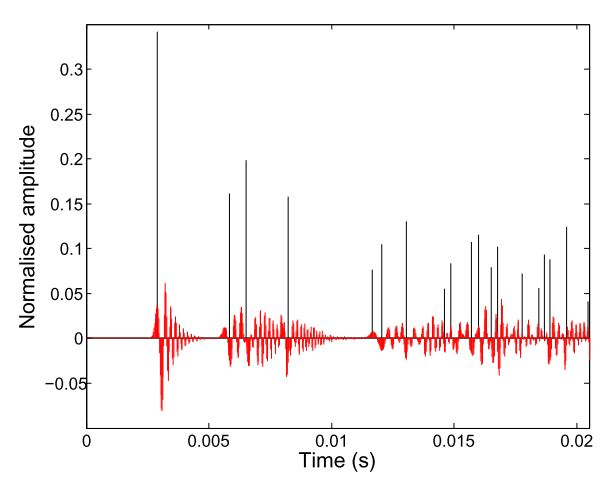
\includegraphics[width=0.75\textwidth]{impulseresponse.jpg}
\centering
\caption{An impulse response with first reflections~\cite{Mourik2013}}
\end{figure}
\horrule{0.5pt} \\[0.4cm] % Thin top horizontal rule
\huge An Experimental Method to Quantify the Impact of Reverb Processing Techniques on Immersive Spatial Audio for Virtual Reality \\ % The assignment title
\horrule{2pt} \\[0.5cm] % Thick bottom horizontal rule
}

\author{Simon Durbridge} % Your name

\date{\normalsize\today} % Today's date or a custom date

\begin{document}

\maketitle % Print the title

%----------------------------------------------------------------------------------------
%	Contents
%----------------------------------------------------------------------------------------

\tableofcontents

%\newpage

%----------------------------------------------------------------------------------------
%	Figures
%----------------------------------------------------------------------------------------

\listoffigures

\newpage

%----------------------------------------------------------------------------------------
%	Abstract
%----------------------------------------------------------------------------------------

%\section{Abstract}

%\newpage

%----------------------------------------------------------------------------------------
%	Introduction
%----------------------------------------------------------------------------------------

\section{Introduction}

Increases in available computing power, and great strides in research and development have brought a new surge of interest to virtual reality (VR) applications. 
With the introduction of improved VR systems, such as Google Jump, Oculus, Vive and facebook360, using both high end computers, and mobile phone technology to provide immersive visualisation; Further steps are being taken to provide users with immersive sound environments~\cite{OculusCo41online}. 
These environments may be created in an  attempt to emulate real places, or to characterise fictional places.\par

A significant part of how humans identify with their surroundings, includes the perception of the reverberant characteristics of the surrounding area~\cite{rumsey2012spatial}. 
Cues such as the timing and strength of early reflections help humans to localize sound sources, as well as how far from the nearest boundaries the perceivers are. 
Some VR application development platforms provide a simplified model for how reverberation behaves in an audio system, lending creedence to the topics as discussed by Begault~\cite{Begault1995}, Rumsey~\cite{rumsey2012spatial}, Blauert~\cite{Blauert1997} and Wiggins\cite{Wiggins2004}.and may be an oversimplification when attempting to create an immersive audio experience that is tending towards the suspension of disbelief\footnote{This report is not intended to explore or discuss the artistic concept of the suspension of disbelief. For a discussion on this, please refer to Holland~\cite{Holland2003}}.\par

The aim of this report is to introduce a testing method, to allow for the evaluation of different reverb simulation methods with respect to immersive VR audio. 
Initially, a basic description of sound localization theory is given. 
To provide context for spatial audio for VR systems, ambisonics is briefly described in relation to binaural decomposition for VR as this is the currently the more popular format. 
Following this, some theory behind reverberation and perception will be discussed.
Finally, a testing framework will be proposed, in which subjects will evaluate different VR environments and reverb algorithms.

\newpage

%------------------------------------------------
\section{Ambisonic Spatial Audio for Virtual Reality}
\subsection{Spatial Perception}

Though  research into spatial audio for VR may have flourished in recent past, the foundation of localization theory remains based on the concepts explored by Rayleigh in 1907~\cite{Blauert1997}. Continued research into the field as matured and evolved understanding of these concepts, and for an in-depth review of auditory localization concepts, please review Blauert~\cite{Blauert1997}. Lateralization is the term given to he human capacity to binaurally (with two ears) localize sounds laterally in the plane of the ears, and is determined by interaural time differences (ITD), phase differences, interaural level differences(ILD), and the physical listening apparatus itself (pinnae, head shape, torso etc).

\begin{figure}[H]
\centering
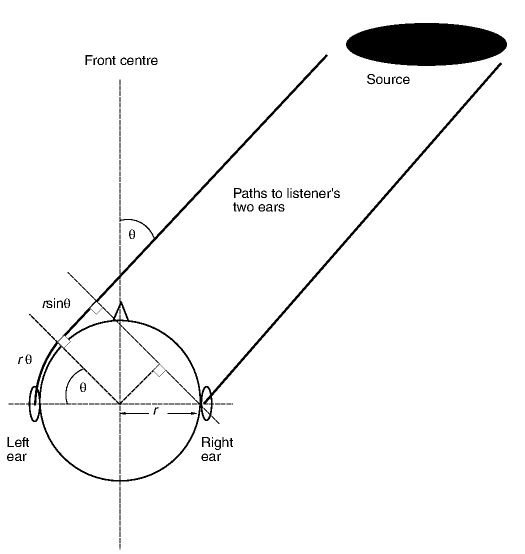
\includegraphics[width=0.4\textwidth]{itdexample.jpg}
\centering
\caption{A basic model diagram of the ITD from a source to a listener given by $\frac{r(\theta + sin \theta)}{\textit{c}}$ ~\cite{rumsey2012spatial}}
\end{figure} 

The ITD is the time difference between a sound arriving at each ear (not to be confused with phase), and is an important cue for localizing at frequencies below the wavelength relative to the size of a listeners head. The phase differences relates tothe asynchronous behaviour of sound diffracting around the head also provides temporally motivated localization cues~\cite{Aaronson2014}. At wavelengths larger than at least half the circumference of the head, sound waves can defract around the head. Above this frequency humans become more dependent of ILDs and phase differences. 

%\begin{figure}[H]
%\centering
%\includemovie[autoplay]{soundwave-to-ears3.gif}
%\end{figure}

The ILD is the level difference between ears of a sound, and is more critical to localization of shorter wavelengths where head and torso shadowing is dominant. The pinnae and torso have a distinct filtering affect that assists humans in localizing sources in the median plane~\cite{Blauert1997}~\cite{Begault1995}~\cite{Wiggins2004}, another benefit of this filtering is that humans are able to some degree overcome the 'cone of confusion' that would occur when a sound source is in a position that would otherwise produce the same ITD and ILD as another position (illustrated below). Another key cue is that humans have a tendency to move their heads, using the changes in what is heard to refine localization~\cite{Blauert1997}.

\begin{figure}[H]
\centering
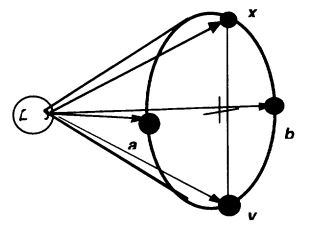
\includegraphics[width=0.4\textwidth]{coneofconfusion.jpg}
\centering
\caption{A diagram example of the cone of confusion. If a source were in location a, it would have the same ITD and ILD and thus would be ambiguous to position b. Positions x and y share a similar relationship in the vertical plane as oposed to the lateral plane of a and b~\cite{Begault1995}}
\end{figure}

The total system of localization effects from source to the entrance of the receivers ear canal(s) can be lumped into a head-related transfer function (HRTF), and can be translated into a head-related impulse response (HRIR). Upon synthesizing an HRIR filter, it is possible to reproduce audio with binaural cues over headphones or an appropriate speaker system, that gives listeners the impression of virtual source localization (and ideally externalization). 

\begin{figure}[H]
\centering
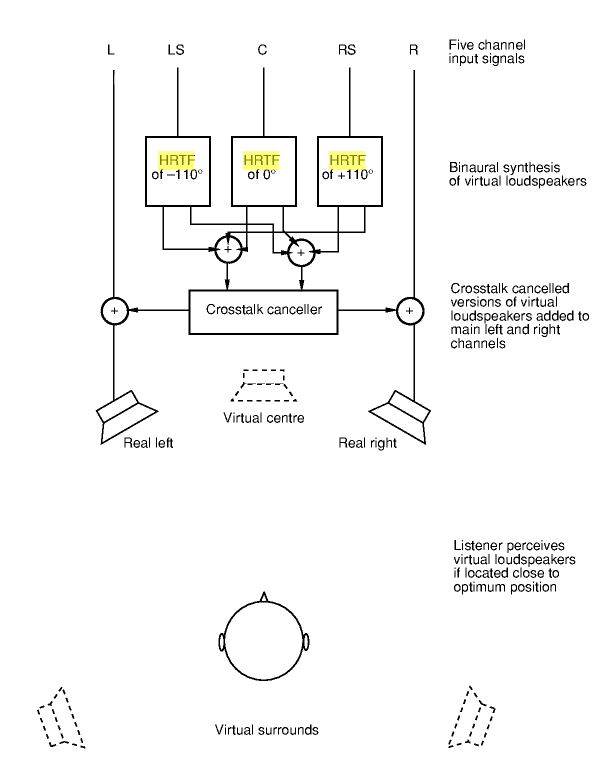
\includegraphics[width=0.6\textwidth]{virtualizationoverspeakers.JPG}
\centering
\caption{A diagram of a loudspeaker system set up for virtualization~\cite{rumsey2012spatial}}
\end{figure}

Auditory Scene Analysis(ASA) is the term given to the brains process of group and compartmentalizing sounds into components of the auditory 'scene'~\cite{rumsey2012spatial}. Through a complex process of continuous analysis and adaptation, the brain is able to accurately differentiate sounds into specific details such as how large a room is, what the wall materials are or which direction a complex source such as an oboe is facing. Bregman~\cite{Bregman1994} suggests that a key part of the ASA process is learned via auditory steaming, which is essentially spectrogram analysis, comparing time and frequency based patterns to those already known, and associating those patterns as another object in the scene. 
\subsection{Ambisonics for virtual reality}

Many of the recent VR systems consist of a viewing headset that may be powered by a mobile phone, a games console or a computer. The headsets viewing system provides a stereoscopic vision of a 3d environment that is linked to a head tracking interface, allowing the user to explore the 'immersive' visual environment in 3d. For many of the new virtual reality platforms, ambisonics has become the signal format of choice. This choice may be due to the flexability of a system that can encode and decode arbitrary numbers of input and output channels, while maintaining a high degree of spatial data. Another benefit may be the compatability of ambisonics with concepts such as object based audio CITE. For a review of various 'spatial' audio system formats, please refer to~\cite{Wiggins2004}. Many of the newer VR platforms rely on headphones as the preferred audio system format. This may be in part due to the difficulty in producing HRTFs for multiple listeners over loudspeaker, though research in this area is continually improving~\cite{Galvez2016}. Another benefit of the use of headphones is that head tracking can be applied to HRTFs to improve the spatial audio quality~\cite{Inanaga1995} in a relatively discrete package.   \\

Ambisonics in a simplistic description, is the spherical harmonic decomposition of a sound field into constituent components~\cite{rumsey2012spatial}. 
That is, by the combination and manipulation of  sets of signals from coincident receivers with figure-of-eight polar responses with an omnidirectional receiver, it is possible to encode a 3 dimensional spatial sound field into an n channel signal format. 
For a discussion on different formats such as B, C, D, A and UHJ, please refer to Rumsey~\cite{rumsey2012spatial}. 
Perhaps the greatest benefit of the ambisonic system is that the encoding and decoding channel counts are not mutually exclusive i.e. it is possible to record a sound field in 3rd order using an appropriate sound-field microphone, and decode that signal for two channel headphone playback with the appropriate HRTFs~\cite{Jot1998} as could be used in a VR system~\cite{Collins2013}. This would allow for multiple virtual sound sources to be used to render a 3d sound field for an individual listener, and could be coupled with head tracking to create an auditory scene that changes as a listeners moves their head.\
\newpage
%------------------------------------------------
\section{Reverberation \&\ Perception}
%---------------------------------------------
\subsection{Reverberation}

The reverberant sound field is the steady-state of diffusely scattered sound energy in a space due to the reflection of that energy from boundaries to a high order. 
Specifically, the amplitude of these reflections are such as to balance in amplitude with the steady state (source - decay) of the acoustic system, at or beyond the critical distance from a source (a classic analogy is given by Everest)~\cite{Everest2009}. 

\begin{figure}[H]
\centering
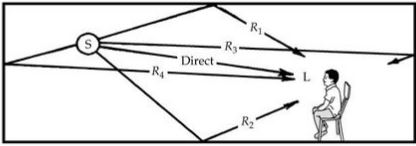
\includegraphics[width=0.4\textwidth]{reflection_diagran.jpg}
\centering
\caption{A conceptualisation of direct and reflected sound~\cite{Everest2009}}
\end{figure}

That is in contrast with low order reflections that may occur before the sound contributes to the reverberant field (early reflections), or may occur later and above the steady state amplitude (echos)~\cite{Everest2009}. 
Early and strong reflections are of significant interest in this study, due to the cues humans receive from perception of them. 
A reverberant sound field is often quantified by the decay time from steady state, to an amplitude of the steady state level $-60{dB}$. This is commonly described as the $RT_{60}$ and was proposed by WC Sabine in 1900. For a discussion of reverb time calculation, please see Everest~\cite{Everest2009} page 153.
The use of $RT_{60}$ as the preferred metric of decay time is valid, assuming that the acoustics system is linear and time-invariant.
A more comprehensive description of reverberation and overview of the associated parameters is given by Rossing~\cite{rossing2007springer}. 

\begin{figure}[H]
\centering
\begin{subfigure}[b]{0.4\textwidth}
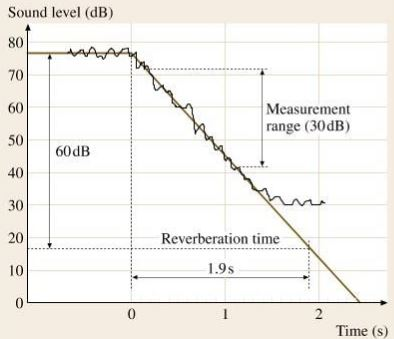
\includegraphics[width=\textwidth]{revertimedefinition.jpg}
\centering
\caption{An example graph of reverberation decay time $RT_{60}$}
\end{subfigure}
~
\begin{subfigure}[b]{0.4\textwidth}
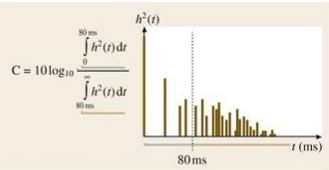
\includegraphics[width=\textwidth]{clarityscore.jpg}
\centering
\caption{An example of the calculation of Clatiry score}
\end{subfigure}
\caption{Graphics pertaining to quantification of reverberant sound ~\cite{rossing2007springer}}
\end{figure}
\newpage

Further to this, the ratio of direct sound amplitude from a source to the amplitude of the reverberant field at any place in the sound field is also of interest~\cite{Begault1995} and is described as the \textbf{D}irect to \textbf{R}everberant (D/R) enegry ratio. This can be quantified in terms of amplitude at a point in the sound field using the modified Hopkins-Stryker equation~\cite{davis2006sound}:\\ 
\begin{center}
$L_T = L_W + 10 log \left( \frac{QMe}{4\pi D_{x}^2} + \frac{4N}{S \overline{a} M a}\right) + K $\\
\end{center}
where:
\begin{enumerate}
\item $L_T =$ total sound pressure
\item $L_W =$ sound power level of source
\item $\frac{QMe}{4\pi D_{x}^2}$ is a description of the sound source direct radiation properties
\item $\frac{4N}{S \overline{a} M a}$ is a description of the reverberant field properties
\item $K = \frac{\rho \textit{c}}{400}$ relating to the transfer of sound through air
\end{enumerate}

This equation is particularly useful, as it can be rearranged to calculate important parameters such as the amplitude of the direct and reverberant sound fields, but also presents the intrinsic relationship between source parameters, receiver location and sound field geometry(including sound absorption properties etc.).
The D/R ratio is intrinsically linked in this equation to the \textbf{critical distance}$(D_c)$, the distance from sound source at which the reverberant sound field is equal in amplitude to direct sound energy from the source. At distances beyond $D_c$ the reverberant sound field dominates the direct sound in amplitude.
A third parameter of interest is the clarity score, that is determined by the ratio between direct sound and an integration of the sound received directly from the source for some arbitrary~\cite{Begault1995} time (commonly 80ms). 
Another parameter of note in calculation of the reverberant nature of a geometry is the mean free path (\textbf{MFP}), that is the average distance between reflections in space~\cite{davis2006sound}:
\begin{center}
$ \textbf{MFP} = 4 \frac{Volume}{Surface area}$
\end{center}
As a wave must propagate further between reflective surfaces, the amplitude of higher order reflections is increasingly diminished. This is compounded by the absorption characteristics of the boundaries of the geometry. Thus, a higher mean free path may result in a reduction in the amplitude of a reverberant tail, compared to a much smaller space with the similar absorption characteristics. 

\newpage

\subsection{Perception of Reflections}
There is a plethora of research and understanding of the objective quantification of reverberation~\cite{rossing2007springer}, less so about the subjective effects~\cite{Karjalainen2001} beyond the seminal studies of early reflections and level threshold shifts by early pioneers (even before Haas)~\cite{Haas1972}. 
It may be argued that many facets of human auditory perception relate in some way to the perception of reverberation, the concepts of interest in this paper are those linked with localisation and perception of the auditory scene. 
Within these concepts are Haas/Precedence effect, and auditory masking.

The Haas effect is described as the first wave-front perceived by a listener, determines the source localisation in an auditory scene. The following reflections received within a 0.7 to 35mS window are integrated with the initial sound, such that the sound is given the impression of increased loudness, an increase in source width and tonal shifts of the percieved sound~\cite{Everest2009}. 
Beyond 40mS, following strong reflections are heard as echoes. 
Begault~\cite{Begault1995} suggests that the precedence effect is the intrinsic mechanism  of the human auditory system, that allows for the localization of sound sources on a reverberant sound-field. 
Begault also suggests that there is a link between inter-aural time difference(ITD) perception for lateralization, and changes in apparent sound source 'width', suggesting a 5us to 1.5ms ITD 'window' within which a sound sources lateral location is determined. Another ascpet of note, is that if a sound source is occluded and the reflected sound is louder than the direct sound, the precedence effect is diminished~\cite{Wiggins2004}.

\begin{figure}[H]
\centering
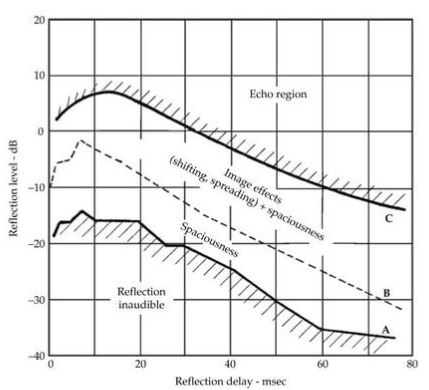
\includegraphics[width=0.4\textwidth]{precedence.jpg}
\caption{A plot of the window regions of precedence between reflection 'level' and delay~\cite{Everest2009}}
\end{figure}

Many of the texts referenced in this section of the report do not discuss auditory masking in great detail\footnote{Masking is noted several times by Begault, but not discussed}, though it may be of considerable importance when considering perception of noise-like sound.
Auditory masking can be conceptualised as the time-envelope dependent blocking of new sounds being perceived, due to some other sound having already excited the inner ear. 
Specifically, sounds having already excited a portion of the bascilar membrane are thus stopping other sounds from being perceived as separate, that would otherwise excite the same portion of the bascilar membrane~\cite{Everest2009}. 
The basilar membrane is often regarded as to be discretized into critical bands or equivalent rectangular bandwidths (ERB), and these bandwidths are different depending on sound level as well as centre frequency. 
General works by Moore ~\cite{Moore1996} should be reviewed for a more in-depth discussion of masking. The relevance of masking in this context, is that continuous noise is often used as a test signal in masking experiments, and steady-state reverberation may be similar to noise and thus cause masking of reflections and general reverberation. As such, creation of realistic reverberation may be important for masking in a natural way as opposed to having a spectrally dense or high amplitude artificial reverb that may cause excessive masking.

Sigfried Linkwitz~\cite{Linkwitz2015} also discussed the idea that human perception of sound in enclosed spaces is powerful enough that given an appropriate pair of sound sources, a person can subconsciously differentiate between reflected sounds and the stereo sound-stage created by the two sound sources. This is not disimilar to abstractions made in much of the literature such as Begault~\cite{Begault1995} or Wiggins~\cite{Wiggins2004}, who describe typical scenarios pertaining to walking into large spaces and using cues from reflections to determine that the space they have entered is actually large. The relevant link between reverberation and associated perceptual faculties is with auditory scene analysis. Reverberation perception (particularly precedence) is intrinsically linked to humans capacity to analyse the auditory characteristics of their surroundings. This is compounded by Begault~\cite{Begault1995} who notes the significant breadth of reverberation research for concert hall acoustics, suggesting that the quality of reverberation may be an important part of audio for VR and multimedia.\\ 
The argument is that more realistic reverberation modelling may provide a more realistic scene for our brains to analyse. In fact it has been shown by Corey~\cite{Corey2002} that for a 5 channel system, adding simulated early reflections are enough to allow listeners to accurately localize sound sources with greater certainty. However, in a similar way some of the VR packages, Corey's early reflections were generated using an image source method. As note in acoustic modelling research such has those by Mourik and Murphy~\cite{Mourik2013}, geometric or ray based simulations do not produce accurate results at low frequencies. The image based method described by Begault~\cite{Begault1995}, and used by Corey is also only usable for rectangular spaces and is limited further. Some reverb calculation methods are discussed in the next section.

\subsection{Synthetic Reverberation Algorithms}
\subsubsection{filter based reverb}

A relatively simple electronic method of simulating reverberation is that derived by a feedback loop. An analogy of this system is that of a tape deck with a looped reel of tape~\cite{Begault1995}. A delay presented between the read and write heads of the tape deck, with the write head writing not only new signals to the tape but an attenuated version of the signal read by the read head producing a decaying echo. In the frequency domain, such a system presents a comb filtered response as a version of a signal is interfering with itself but staggered in time.\\ 

When a series of these reverberation filters are cascaded together with varying delay times, it is possible to create a slightly metallic sounding reverb CITE FREVERB. An improvement to this method is to add a signal to itself with the same delay, however one version of the signal has been passed through a flex frequency all-pass filter that warps the phase response of the signal. A series of these devices cascaded together will also produce a reverb effect.\\

A third method of creating a reverb effect is to convolve a signal with the finite impulse response (FIR) impulse response of the system to be emulated, or with a decaying 'shaped' noise function. This process in discrete digital systems involves multiplying a current sample and $n-1$ previous samples with $n$ coefficients, thus adding varying amounts of the previous portion of the signal to the 'current' sample. This method is also required for digitally applying the measured impulse response of a real space to some audio for simulation purposes, and the same again for a modelled or calculated impulse response using one of the modelling techniques discussed below. 

\subsubsection{modelling}
Geometric based modelling methods are those based on assumptions of plane wave propagation and ray based geometry to calculate the time of flight and  of some sound between a source and a receiver. These methods include image source modelling, ray tracing, cone tracing and various other variations~\cite{Elorza2005}. This report will focus on the previously mentioned image source technique.\\

The image source(IM) technique uses a rectilinear geometry with some basic frequency-independent absorption characteristic, and conceptually multiplies that geometry in symmetric fashion around the origin geometry. The effective time of flight and number of virtual boundaries passed indicates some absorption, reflection order and time delay between the source and receiver. Thus, the impulse response of the geometry can be calculated with accuracy up to the order of the simulation i.e. how many times the geometry is mirrored. This method cannot handle an irregularly shaped geometry, any obstacles, and assumes that the ray represents part of a plane wave whose wavelength is much smaller than any part of the geometry. This method is however relatively simple, fast to compute and is potentially a good method for calculating arrival times and amplitudes of early reflections for a binaural pair of receivers down to the rooms Schroeder frequency.

Using the calculated reverb decay time $RT_{60}$ to set up an IIR reverb and the early reflection results from an IM simulation, it is potentially possible to combine the two responses to create and artificial reverberation for VR environments that provides early reflections for localization, but is not to such a high order as to become computationally expensive. \\

Wave based modelling methods directly model spaces by calculating solutions to a discretized partial differential equation across the geometry. For linear and room acoustics, the equation used is often the linearised Navier-Stokes or Euler diffusion style equations that satisfy the conservation laws. Depending on the solving scheme used, the geometry will need to be discretized to at least 2 points per wavelength (in line with Nyquist theorem) and potentially beyond 10 points\footnote{particularly for explicit finite different and finite element methods} per wavelength to satisfy the Courant condition. The result is that problems become exponentially large and thus expensive to solve up to high frequencies. However, some methods such as the PTSD have been used to calculate up to low-mid frequencies in real time and may in future become suitable to calculating low frequency portions of hybrid models in VR.

%----------------------------------------------------------------------------------------
\newpage
\section{Experiment Protocol}
\subsection{experiment aims}
The aim of subsequent research to this report, is to define how much of an impact the accuracy of reverberation synthesis has on the perception of a space in a VR application. Is there a direct correlation between the order of accuracy of a simulation, and test subjects believing the space they are hearing is real or at least realistic. 

\subsection{experiment method}
Users will be asked to evaluate 3 different listening environments, with a speech stimulus of two people talking in the space. There will be five potential reverb scenarios to evaluate in each environment: 
\begin{itemize}
\item convolving with an real IR of a real space
\item a derived reverb
\item a low order image source IR combined with a derived reverb
\item a high order image source IR
\item a control instance of the signal with the IR of a real place
\end{itemize}
Subjects will be asked to perform an evaluation test in which they use a simple VR headset and headphones to evaluate a space in VR. Subjects will be able to look around the scene, but not move from that position within it. The subjects will be asked to identify on a paper form, in which directions the people speaking are situated. Test material will be predetermined by either youtube video Subjects will be shown an initial 'training' scene, that will prepare them for the upcoming stimulus, but the test will be blind to what is being tested for until the post-test debrief. The test will be taken in real-world conditions i.e. in variable environments and with non-strict hardware conditions, this is to ground the experiments to scenarios where these basic VR systems are intended to be used. The results will then be analysed for accuracy i.e. which auditory scenes and images or spaces were correctly matched.

Karjalainen \textit{et al}~\cite{Karjalainen2001} undertook a study into the perception of late reverberation, using a perceptual model to reinforce listening test data.

\section{Conclusion}
The intention of this paper was to explore some of the key psychoacoustic and physical principals behind the localization of sounds in relation VR, so that a listening test may be designed for evaluating the effect of different reverb synthesis methods on localization. 

%----------------------------------------------------------------------------------------
\newpage
\section{References}

\bibliography{mylibrary}{}
\bibliographystyle{plain}

\end{document}